%%
%% This is file `sample-manuscript.tex',
%% generated with the docstrip utility.
%%
%% The original source files were:
%%
%% samples.dtx  (with options: `manuscript')
%% 
%% IMPORTANT NOTICE:
%% 
%% For the copyright see the source file.
%% 
%% Any modified versions of this file must be renamed
%% with new filenames distinct from sample-manuscript.tex.
%% 
%% For distribution of the original source see the terms
%% for copying and modification in the file samples.dtx.
%% 
%% This generated file may be distributed as long as the
%% original source files, as listed above, are part of the
%% same distribution. (The sources need not necessarily be
%% in the same archive or directory.)
%%
%% The first command in your LaTeX source must be the \documentclass command.
\documentclass[manuscript,screen]{acmart}
\usepackage{graphicx}
\graphicspath{ {./images/} }
\usepackage{fancyvrb}
\usepackage{multirow}
\usepackage[section]{placeins}
\usepackage{flafter}
%%
%% \BibTeX command to typeset BibTeX logo in the docs
\AtBeginDocument{%
  \providecommand\BibTeX{{%
    \normalfont B\kern-0.5em{\scshape i\kern-0.25em b}\kern-0.8em\TeX}}}

%% Rights management information.  This information is sent to you
%% when you complete the rights form.  These commands have SAMPLE
%% values in them; it is your responsibility as an author to replace
%% the commands and values with those provided to you when you
%% complete the rights form.
\setcopyright{acmcopyright}
\copyrightyear{2022}
\acmYear{2022}
%\acmDOI{10.1145/1122445.1122456}

%% These commands are for a PROCEEDINGS abstract or paper.
\acmConference [RecSys'22] 
{Seattle, WA USA}
{16th ACM Conference on Recommender Systems, Seattle, WA USA, Sept. 18 - 23, 2022}

\acmBooktitle{16th ACM Conference on Recommender Systems,  Seattle, WA USA, Sept. 18 - 23, 2022}

\acmPrice{15.00}
\acmISBN{978-1-4503-XXXX-X/18/06}


%%
%% Submission ID.
%% Use this when submitting an article to a sponsored event. You'll
%% receive a unique submission ID from the organizers
%% of the event, and this ID should be used as the parameter to this command.
%%\acmSubmissionID{123-A56-BU3}

%%
%% The majority of ACM publications use numbered citations and
%% references.  The command \citestyle{authoryear} switches to the
%% "author year" style.
%%
%% If you are preparing content for an event
%% sponsored by ACM SIGGRAPH, you must use the "author year" style of
%% citations and references.
%% Uncommenting
%% the next command will enable that style.
%%\citestyle{acmauthoryear}

%%
%% end of the preamble, start of the body of the document source.
\begin{document}

%%
%% The "title" command has an optional parameter,
%% allowing the author to define a "short title" to be used in page headers.
\title{Evaluating the Accuracy and Coverage Performance of Collaborative Filtering, Content-Based, and Hybrid Recommender Systems}

%%
%% The "author" command and its associated commands are used to define
%% the authors and their affiliations.
%% Of note is the shared affiliation of the first two authors, and the
%% "authornote" and "authornotemark" commands
%% used to denote shared contribution to the research.

\author{Anh Hoang}
\affiliation{%
  \institution{Davidson College}
  \streetaddress{102 N Main Street}
  \city{ Davidson}
  \state{ North Carolina}
  \postcode{ 28035}
  \country{USA} }
\email{duhoang@davidson.edu}

\author{Malavika Kalani}
\affiliation{%
  \institution{Davidson College}
  \streetaddress{102 N Main Street}
  \city{ Davidson}
  \state{ North Carolina}
  \postcode{ 28035}
    \country{USA} } 
\email{makalani@davidson.edu}

\author{Mike Remezo}
\affiliation{%
  \institution{Davidson College}
  \streetaddress{102 N Main Street}
  \city{ Davidson}
  \state{ North Carolina}
  \postcode{ 28035}
    \country{USA} } 
\email{miremezo@davidson.edu}



%%
%% By default, the full list of authors will be used in the page
%% headers. Often, this list is too long, and will overlap
%% other information printed in the page headers. This command allows
%% the author to define a more concise list
%% of authors' names for this purpose.
\renewcommand{\shortauthors}{NAMES: Anh Hoang,  Mike Remezo, Malavika Kalani}

%%
%% The abstract is a short summary of the work to be presented in the
%% article.
\begin{abstract}

Recommender Systems is a popular information filtering technology that lends itself to the e-commerce industry due to its usefulness in providing recommendations for consumers and increasing business revenue. There has been substantial research into different types of recommender systems and their implementations. In this paper, we present a comparative study of the three major paradigms of recommender systems: collaborative filtering, content-based, and hybrid methods. We used the MovieLens\cite{movie} data set for our analysis and based our results on two metrics, accuracy and coverage. Our findings reveal that collaborative filtering using matrix-factorization stochastic gradient descent is the best performing algorithm. 

\end{abstract}

%%
%% The code below is generated by the tool at http://dl.acm.org/ccs.cfm.
%% Please copy and paste the code instead of the example below.
%%
%\begin{CCSXML}
%<ccs2012>
% <concept>
%  <concept_id>10010520.10010553.10010562</concept_id>
%  <concept_desc>Computer systems organization~Embedded systems</concept_desc>
%  <concept_significance>500</concept_significance>
% </concept>
% <concept>
%  <concept_id>10010520.10010575.10010755</concept_id>
%  <concept_desc>Computer systems organization~Redundancy</concept_desc>
%  <concept_significance>300</concept_significance>
% </concept>
% <concept>
%  <concept_id>10010520.10010553.10010554</concept_id>
%  <concept_desc>Computer systems organization~Robotics</concept_desc>
%  <concept_significance>100</concept_significance>
% </concept>
% <concept>
%  <concept_id>10003033.10003083.10003095</concept_id>
%  <concept_desc>Networks~Network reliability</concept_desc>
%  <concept_significance>100</concept_significance>
% </concept>
%</ccs2012>
%\end{CCSXML}
%
%\ccsdesc[500]{Computer systems organization~Embedded systems}
%\ccsdesc[300]{Computer systems organization~Redundancy}
%\ccsdesc{Computer systems organization~Robotics}
%\ccsdesc[100]{Networks~Network reliability}

%%
%% Keywords. The author(s) should pick words that accurately describe
%% the work being presented. Separate the keywords with commas.
\keywords{Recommender Systems, Collaborative Filtering, Similarity and Prediction techniques}


%%
%% This command processes the author and affiliation and title
%% information and builds the first part of the formatted document.
\maketitle

\section{Introduction}

\subsection{Definition of Recommender Systems}

Due to technological advancements, the e-commerce industry has witnessed drastic growth in recent decades. Individuals now spend the majority of their time on the Internet. However, given the overwhelming number of choices available online, there is a potential risk of information overload for many Internet users. Recommender systems offer solutions to this particular problem. 

Recommender systems are personalized information filtering technology employed to make predictions on the potential likeness of users towards different products and provide them with recommendations for a set of items that are of interest to them. On the users’ side, given the wide availability of products online, recommender systems solve the problem of how to filter, prioritize, and efficiently deliver suggestions on items that best fit consumers’ needs, reducing the risks of information overload and increasing users’ satisfaction. On the service provider’s side, effective recommender systems can increase revenue and build consumers’ loyalty to the business. 

\subsection{How Does A Recommender System Work?}

In essence, a recommender system strives to predict the rating or potential preference that a user would give an item. Once the system outputs a prediction, recommendations will be given to users. Building a recommender system consists of three steps: retrieving users’ data and formatting it for manipulation, computing similarity among users or items, and performing predictions of unknown ratings for users\cite{par}. Users’ data can be retrieved implicitly or explicitly\cite{par}. Explicit data includes users’ ratings and feedback, whereas implicit data can be congregated from users’ purchase history, the number of clicks on certain items, and the likes\cite{par}. Data will then be formatted; one common way to do so is to convert a user-item matrix into a rating matrix. 

\subsection{Types of Recommender Systems}

Recommender systems can be categorized into three main types: Collaborative filtering, Content-based filtering, and Hybrid methods\cite{par}. 

Collaborative filtering is an algorithm that generates recommendations for a user through a systematic analysis of data collected from other users sharing similar tastes or information needs\cite{par}. Collaborative filtering can be broken down into memory-based methods and model-based methods\cite{par}.

Memory-based methods, also known as neighbourhood-based methods, are methods where the predictions of whether a user will like an item or not, can be computed using the information of their neighbours\cite{par}. There are two main branches of memory-based methods: User-based collaborative filtering (UBCF) and item-based collaborative filtering (IBCF)\cite{par}. UBCF focuses on finding people who like the same items as the active user and recommending items that those people like, while in IBCF,  the similarities among items are calculated and the unrated items with high similarity will be recommended to users\cite{par}. The core recommending algorithm can be broken down into three steps for both user-based and item-based methods: 
\begin{enumerate}
    \item Apply different weightings to all users/ items to calculate the similarity among users and items
    \item Create a subset of users/items to predict the ratings for an item that the user has not rated 
    \item Perform normalization of ratings and calculate the prediction using a weighted array of selected neighbours’ ratings\cite{her99}. 
\end{enumerate}

For model-based methods, the algorithms are built on the latent factor models\cite{koren}. Latent factor models seek to characterize both items and users on factors that can be inferred from the rating patterns\cite{koren}. One of the most successful latent factor models uses matrix factorization, which characterizes both items and users through vectors of factors that are computed from the item rating patterns\cite{koren}. Matrix factorization models map both users and items to a joint latent factor space, and user-item interactions are the inner products of corresponding vectors in the space\cite{koren}. To find out the factor vectors, the system minimizes the regularized squared error on the set of known ratings\cite{koren}. The system will try to learn the model by fitting the previously observed ratings.

Content-based filtering is a recommender algorithm that recommends items based on the attributes of the items themselves\cite{par}. First, the algorithm will generate content information for items. Then, it will produce user-profiles and preferences with regard to features of the product\cite{pazz}. Finally, it looks for items that are similar to the items that users have liked in the past by analyzing items’ descriptions and features\cite{pazz}. 

Hybrid methods are recommender algorithms that combine both content-based filtering and collaborative filtering methods to maximize their strengths and minimize their weaknesses\cite{par}. There are multiple approaches to building a hybrid model. A notable example is combining separate recommenders, where we will use a linear combination of ratings or a voting scheme, or switch between the two after analyzing which one is better at any given moment\cite{adoma}. Another popular approach is to add content-based characteristics to collaborative filtering methods, where we keep content-based profiles to aid with the collaborative filtering process, which helps with reducing sparsity and the algorithm will be able to recommend items directly similar to the user's taste\cite{adoma}.


\subsection{Our Goal}

In light of the substantial number of existing recommender systems models, we seek to explore which model performs the best. Therefore, our paper presents an empirical analysis  of collaborative filtering, content-based, and hybrid recommender systems; ultimately, our goal is to propose the best recommendation algorithm based on metrics that will be defined in our thesis section.



%%Introduce your work effort here. Explain the motivation for undertaking this work and the importance to the Recommender System field. Include a brief discussion of research questions to be pursued/answered in this study. Indicate any novel approaches.



\section{Related Work}
%%This section presents the prior work that has been conducted in this area of research. Use citations and the accomplishments of the prior work.
In this section, we briefly present some of the research literature related to the implementations of the collaborative filtering system, , content-based and hybrid systems. 
Recommender systems have become a popular system that most companies and platforms rely on for offering a reliable and personalized experience to a user by providing the best recommendations. 
\newline
	User-based collaborative filtering systems predict the rating of an item by a user based on the ratings of other users who are similar to the active user. A common problem with user-based neighborhood recommendation systems is that it does not take into account that the similar users to the active users can have different levels of similarity.One way to address this problem is to apply similarity weighting to each contribution of each similar user \cite{des} . Our research uses this idea of similarity weighting for our recommendations produced by the user-based collaborative filtering system. 
	\newline
	 There are two categories of collaborative filtering algorithms: memory-based which utilizes the entire user-item database to generate a prediction and model-based which provides item recommendation by developing a model of user ratings \cite{bad}. 
	Matrix factorisation technique is another approach to producing recommendations that we have explored in our paper. It characterizes both items and users by vectors of factors inferred from item-rating patterns. In order to minimize the regularized squared error, there are two popular methods known as stochastic gradient descent and alternating least squares \cite{koren}. Stochastic gradient descent algorithm loops through all the ratings in the training set and alternating least squares rotates between fixing the item and user vectors which ensures that the squared error minimizes until it becomes really small. The accuracy and performance of both these methods have been detailed in our research. 
\newline
	Content-based recommendation system is another approach that analyzes item descriptions and features to identify items that might be worthy of a recommendation to a user \cite{adoma} . Unstructured data such as unrestricted text items cannot be described by a set of attributes. A process of stemming is used to create a term that reflects the common meaning behind similar words \cite{adoma} . The value of the variable related to the term is known as term-frequency times inverse document frequency (or tf-idf) which denotes the frequency of a term in a document, the number of documents that contain that term and the total number of documents in the collection.
An important limitation of content-based systems using feature encoding is that the features of the recommended items must be easily parsed or assigned to items \cite{adoma} . Additionally, hybrid approaches produce more accurate recommendations in comparison to pure approaches \cite{adoma}. We have analyzed our results for such hybrid systems using  item-based collaborative filtering approach combined with content-based TF-IDF technique. 
Lastly, our analysis of different hybrid recommender models is greatly aided by the comprehensive view of in-depth examples of different hybrid models and the discussion of benefits and drawbacks provided in \cite{burke}. 
				


\section{Thesis}
%%This section explains the research that will be performed in this work (WHAT), 
%%details of the motivation behind this effort (WHY), 
%%a discussion of the Hypotheses that will be tested (EXPECTED RESULTS),
%%and a brief description of how the research effort will be conducted (HOW). 
%%Use formulae and/or equations to detail the math behind this effort.
In this section, we will describe the research that we performed in this work and its main objective. We will also provide a brief description of how the research was conducted along with important details regarding the mathematical ideas and formulae used.  Several algorithms and approaches have been explored to build a strong recommendation system for users to have a better experience while also managing the increasing load of user information.  Our research aims to apply variations of parameters on the different algorithms implemented under collaborative filtering systems, model-based methods using matrix factorization, content-based filtering and hybrid recommendation systems. For each kind of recommender system, we will be analyzing the results produced by each algorithm using the best set of parameters. The goal of our research is to determine the best recommender system, one with the maximum coverage and highest accuracy. The metrics used in our experiment to evaluate the quality of each recommender system algorithm can be explained in the following way: 
\begin{enumerate}
    \item Coverage: Coverage denotes the percentage of items for which the recommender system can compute predictions. In our experiment, coverage is shown as the number of items in place of a percentage value. It is desirable to have the maximum coverage as it implies that the prediction provided was computed based on almost all the item ratings existing in the dataset\cite{her99}.
    \item Accuracy: In our experiment, the accuracy of the predictions provided by a recommender system algorithm is evaluated using certain error metrics. For all the error metrics used in our experiment, the lowest error indicates the highest accuracy.The formula for the main error metric used in this paper is shown below:
    \newline
        Mean Squared Error (MSE): The formula for calculating MSE where $n$ denotes the number of ratings, $Y_{i}$ denotes the actual rating and $\overline{Y_{i}}$ demotes the predicted rating is the following:
        \begin{equation}
            MSE = \frac{1}{n}\sum_{i=1}^{n}(Y_{i} - \overline{Y_{i}})^2
        \end{equation}
\end{enumerate}

The two approaches used in our experiment to calculate our accuracy based on MSE are as follows:
\begin{enumerate}
    \item Leave-One-Out-Cross-Validation (LOOCV): For each rating in the user-item matrix, we remove one rating (which constitutes our test data) and use the train data predict our removed rating. Then, we store the squared error between our actual and predicted rating and restore the removed rating. 
    \item Test/Train Holdout error: This approach divides the actual ratings matrix into test and train sets. For both SGD and ALS, a grid search of runtime parameters is conducted to determine the sets of parameters that best minimize the error between the predicted and actual ratings of the test set. \cite{car}
\end{enumerate}

\subsection{User-based and Item-based Collaborative Filtering }
For each of the user-based and item-based methods, we will be producing results using the following similarity weighting measures: 
\begin{enumerate}
\item \emph{Euclidean distance for recommender systems} calculates the similarity between any two users across all the items they have rated in common. In recommender systems, the \emph{euclidean distance} is a value ranging between $0$ and $1$ where $0$ indicates no similarity and $1$ indicates high similarity. The formula for calculating similarity between the ratings of two users $(u_1, u_2)$ for two items $(i_1,i_2)$ using euclidean distance is shown below:
\begin{equation}
  \emph{Euclidian similarity distance} = \frac{1}{1+\sqrt{(u_1.i_1 - u_2.i_1)^2 + (u_1.i_2-u_2.i_2)^2}}
\end{equation}
\item \emph{Pearson Correlation} also calculates the similarity between two users across all the items they have rated in common. The \emph{pearson correlation coefficient} is a value ranging between $-1$ and $+1$. A value of $-1$ indicates a negative correlation; a value of $1$ indicates high similarity and $0$ indicates no similarity. The formula for calculating similarity between ratings of two users $X$ and $Y$,where $\overline{X}$ and $\overline{Y}$ denote the respective average of their ratings, is shown below: 
\begin{equation}
  \emph{Pearson Correlation between user X and user Y} = \frac{\sum_{i=1}^{n}(X_i - \overline{X})(Y_i - \overline{Y})}{\sqrt{\sum_{i=1}^{n}(X_i - \overline{X})}\sqrt{\sum_{i=1}^{n}(Y_i - \overline{Y})}}
\end{equation}
\end{enumerate}
\hspace{\parindent} A common drawback of the collaborative filtering system is that an active user could have high correlation with other users based on very few commonly rated items between them. The computed correlation between two users does not accurately represent their true correlation if we only have a few data points to compare their item ratings. The accuracy of the predictions could be improved if we can apply a significance weighting measure in the following way: if the number of commonly rated items ($n$) between the two users is less than a weight $w$ then we can apply a significance weight of $n/w$. If the number of commonly rated items ($n$) between two users is more than the weight, then we apply a weight of $1$ \cite{her99}. The significance weights help us devalue the similarity weights that were based of fewer commonly-rated items as described in  \cite{her99}. Ultimately, this enables us to produce a more reliable correlation between two users. For our experiment. we have applied the following significance weight variations to each of our user-based and item-based processes for each similarity measure (euclidean distance and Pearson):
\begin{enumerate}
\item significance weight of $1$
\item significance weight of $n/25$ where $n$ is the commonly rated items
\item significance weight of $n/50$ where $n$ is the commonly rated items
\end{enumerate}
\hspace{\parindent} In addition to applying the significance weights, it is crucial to choose the specific users whose ratings can be used in computing the predicted rating of the active user. As explained in  \cite{her99}, it is more accurate to use a subset of other similar users instead of the entire database to generate a prediction for the active user. For large-scale collaborative filtering recommender systems, it is time-consuming to use the entire user database to generate predictions. This is why it is important to selectively choose the best set of users to compute a prediction for the active user. As explained in  \cite{her99}, we have implemented the absolute threshold technique in our experiment. According to this method, we create our subset of other users by selecting only those users whose absolute correlation with the active user is greater than our given threshold. For our experiment. we have applied the following threshold values to each of our user-based and item-based processes for each similarity measure (euclidian distance and pearson):
\begin{enumerate}
\item threshold = $0$
\item threshold = $0.3$
\item threshold = $0.5$
\end{enumerate}

\hspace{\parindent} After choosing the best subset of other users, their ratings are utilised to compute a prediction for the active user. \cite{car}

\newline 

\subsection{Collaborative Filtering using matrix factorisation}
Matrix factorisation algorithms work by decomposing the user-item interaction matrix into the product of two lower dimensional rectangular matrices. 

Generally speaking, each item $i$ is associated with a vector $q_{i}$ and each user $u$ is associated with a vector $p_{u}$. To learn the latent vectors, the matrix factorisation system minimises the MSE on the set of known ratings: $min_{q^*,p^*} = \sum_{(u,i) \in K} (r_{ui} - p_{u}q_{i}^{T})^2$ where k is the set of the (u,i) pairs for which $r_{ui}$ is known.
The following mathematical equations were used for the system to learn the latent factors by minimizing the MSE: \cite{car}
\begin{enumerate}
    \item usng SGD: $min_{q^*,p^*} = \sum_{(u,i) \in K} (r_{ui} - p_{u}q_{i}^{T})^2 + \lambda(||q_i||^2 + ||p_i||^2 + b_u^2 + b_i^2)$ where $b_u$ and $b_i$ represent user and item bias components and $\lambda$ is the regularisation term.
    \item using ALS: $min_{q^*,p^*} = \sum_{(u,i) \in K} (r_{ui} - p_{u}q_{i}^{T})^2 + \lambda(||q_i||^2 + ||p_i||^2$ where $\lambda$ is the regularisation term. 
\end{enumerate}
For our experiment, we have analysed the following parameters with SGD:
\begin{enumerate}
    \item number of latent features: $2, 20, 200$
    \item learning rate: $0.02, 0.002,0.0002$
    \item regularization term: $0.2, 0.02, 0.002$
\end{enumerate}
\newline We have analyzed the following parameters with ALS:
\begin{enumerate}
    \item number of latent features: $2, 20, 100, 200$
    \item regularization term: $1.0,0.1,0.01,0.001,0.00001$
\end{enumerate}


\subsection{Content-based methods: FE and TFIDF}
Feature encoding turns categorical data in a dataset into numerical data. In case of our dataset ML-100K, feature encoding algorithm acquires the item-features' given domain. Then, we generate recommendation data by creating a preference matrix based on feature profiles of movies the user has seen and rated. The recommendations are computed for movies not yet rated by the user based on the feature profiles and the user preference matrix. The sum of the weighted preferences vectors are normalised to produce weights. A recommendation is computed by the sum of the product of the weights and user ratings: predicted rating $= \sum weights*(\text{user ratings})$. It is important to note that there is no similarity threshold for the FE algorithm. \cite{car}
\newline Term frequency-inverse document frequency encodes text documents in multi-dimensional Euclidean space as weighted term vectors. In essence, the term frequency measures how often a term appears. It assumes that important terms should appear more often. Additionally the inverse document frequency aims to reduce the weight of terms that appear in all documents (common, may be high frequency). $TF(i,j)$ denotes the term frequency of keyword $i$ in document $j$ and $IDF(i)$ is calculated as $log \frac{N}{n(i)}$ where $N$ is the number of documents and $n(i)$ is the number of documents from $N$ in which keyword $i$ appears. Cosine similarity metric is used to compare vectors by computing the angle between them. The algorithm used for our experiment can be explained in the following steps: \cite{car}
\begin{enumerate}
    \item in the cosine similarity matrix, select the similarities between the item the active user has not rated and all the other items (i.e. similar items) the active user has rated.
    \item for every similar item, calculate the product of the rating and the similarity to them item that has not been rated. 
    \item Compute the sum of the products and divide by the sum of all the similarities to the item not yet rated to generate a prediction. \cite{car}
\end{enumerate}
For our experiment, we use $0, 0.3, 0.6, 0.9$ as our threshold variations for TF-IDF. Those threshold values were chosen based on the distribution of the cosine matrix that had a similar shape to a bell curve(fig 1).

\subsection{Hybrid systems}
For our experiment, we are using the TF-IDF system using the cosine similarity matrix as our base recommender system approach combined with an item-based collaborative filtering similarity matrix (using both euclidean distance and Pearson). When the TF-IDF similarity is zero, we look for the corresponding value in the item-item similarity matrix multiplied by a weighting factor of $25\%, 50\%, 75\%$ or $100\%$. \cite{car}

\subsection{Hypothesis}

Implementing the mathematical concepts and algorithms described above, we hypothesize that MF-SGD should be the best performing algorithm based on accuracy and coverage. Matrix factorization algorithm allows for the incorporation of a much more in-depth dataset of information: explicit feedback, implicit feedback, biases, dynamics along with confidence levels\cite{koren}. The prediction of calculation is based on more subtle and complex feature dimensions that user-based or item-based collaborative filtering methods won't be able to spot. Furthermore, we predict that SGD will outperform ALS since ALS is more equipped to deal with a dataset that contains substantial implicit feedback, which is not the case with ML-100k. 

%%This section lays out the assumptions and variations of the study. What datasets were used. What variables will be varied and the extent to which they will be varied. Etc.\\
\section{\textbf{Experiemental Design}}

\subsection{\textbf{Datasets}}
For our experiment, we used the ML100k data from MovieLens\cite{movie}. There are a total 943 users, 1664 movies, and 99693 ratings in this dataset\cite{movie}. Ratings are provided in the range of 1 to 5\cite{movie}. 

\newpage
\subsubsection {\textbf{Layout of dataset statistics}}
% -- Total number of users, items, ratings
% -- Overall average rating, standard dev (all users, all items)
% -- Average item rating, standard dev (all users)
% -- Average user rating, standard dev (all items)
% -- Matrix ratings sparsity
% -->> Average number of ratings per user, standard dev (all users)
% -->> Min, Max, Median number of ratings per user
% -- Ratings distribution histogram (all users, all items) figure.

% Popular items analytics data/Chart for ml-100K: 
% -- popular items: most rated (sorted by # ratings)
% -- popular items: highest rated (sorted by avg rating)
% -- popular items: highest rated items that have at least a "threshold" number of ratings
Descriptive analytics data/Chart for ml-100K:
\vspace{1mm}
\newline
Number of users: 943
\newline
Number of items: 1664
\newline
Number of ratings: 99693
\newline
Overall average rating: 3.53 out of 5, and std dev of 1.13
\newline
Average item rating: 3.08 out of 5, and std dev of 0.78
\newline
Average user rating: 3.59 out of 5, and std dev of 0.44
\newline
User-item Matrix Sparsity: 93.65\%
\newline
Average number of ratings per users: 105.718982, and std dev of 100.567291  
\newline
Min, Max, Median number of ratings per users: 20, 737, 65
\newline
Average number of ratings per items: 59.453032, and std dev of 80.359947
\newline
Min, Max, Median number of ratings per item: 1, 583, 27

\vspace{2mm}
\subsection{Charts}
    \begin{figure}[H]
        \centering
        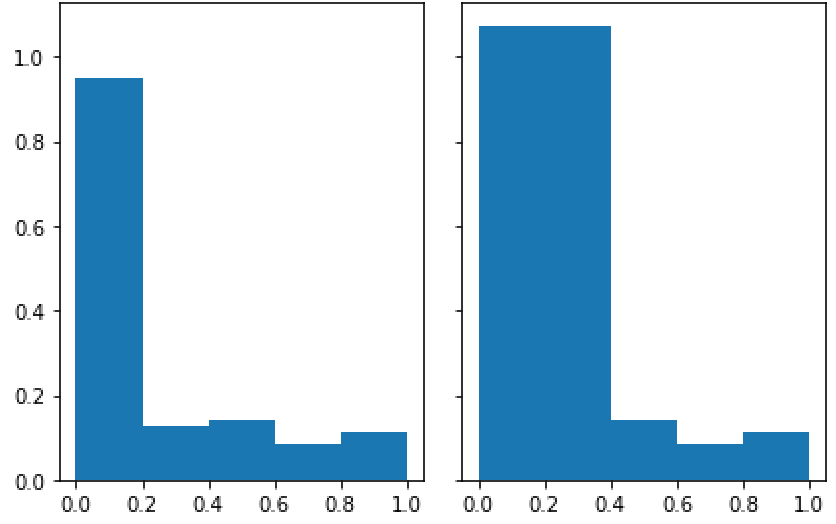
\includegraphics[width=5in]{cosine.png}
        \caption{cosine similarity distribution}
        \Description{}
    \end{figure} 
    \begin{figure}[H]
        \centering
        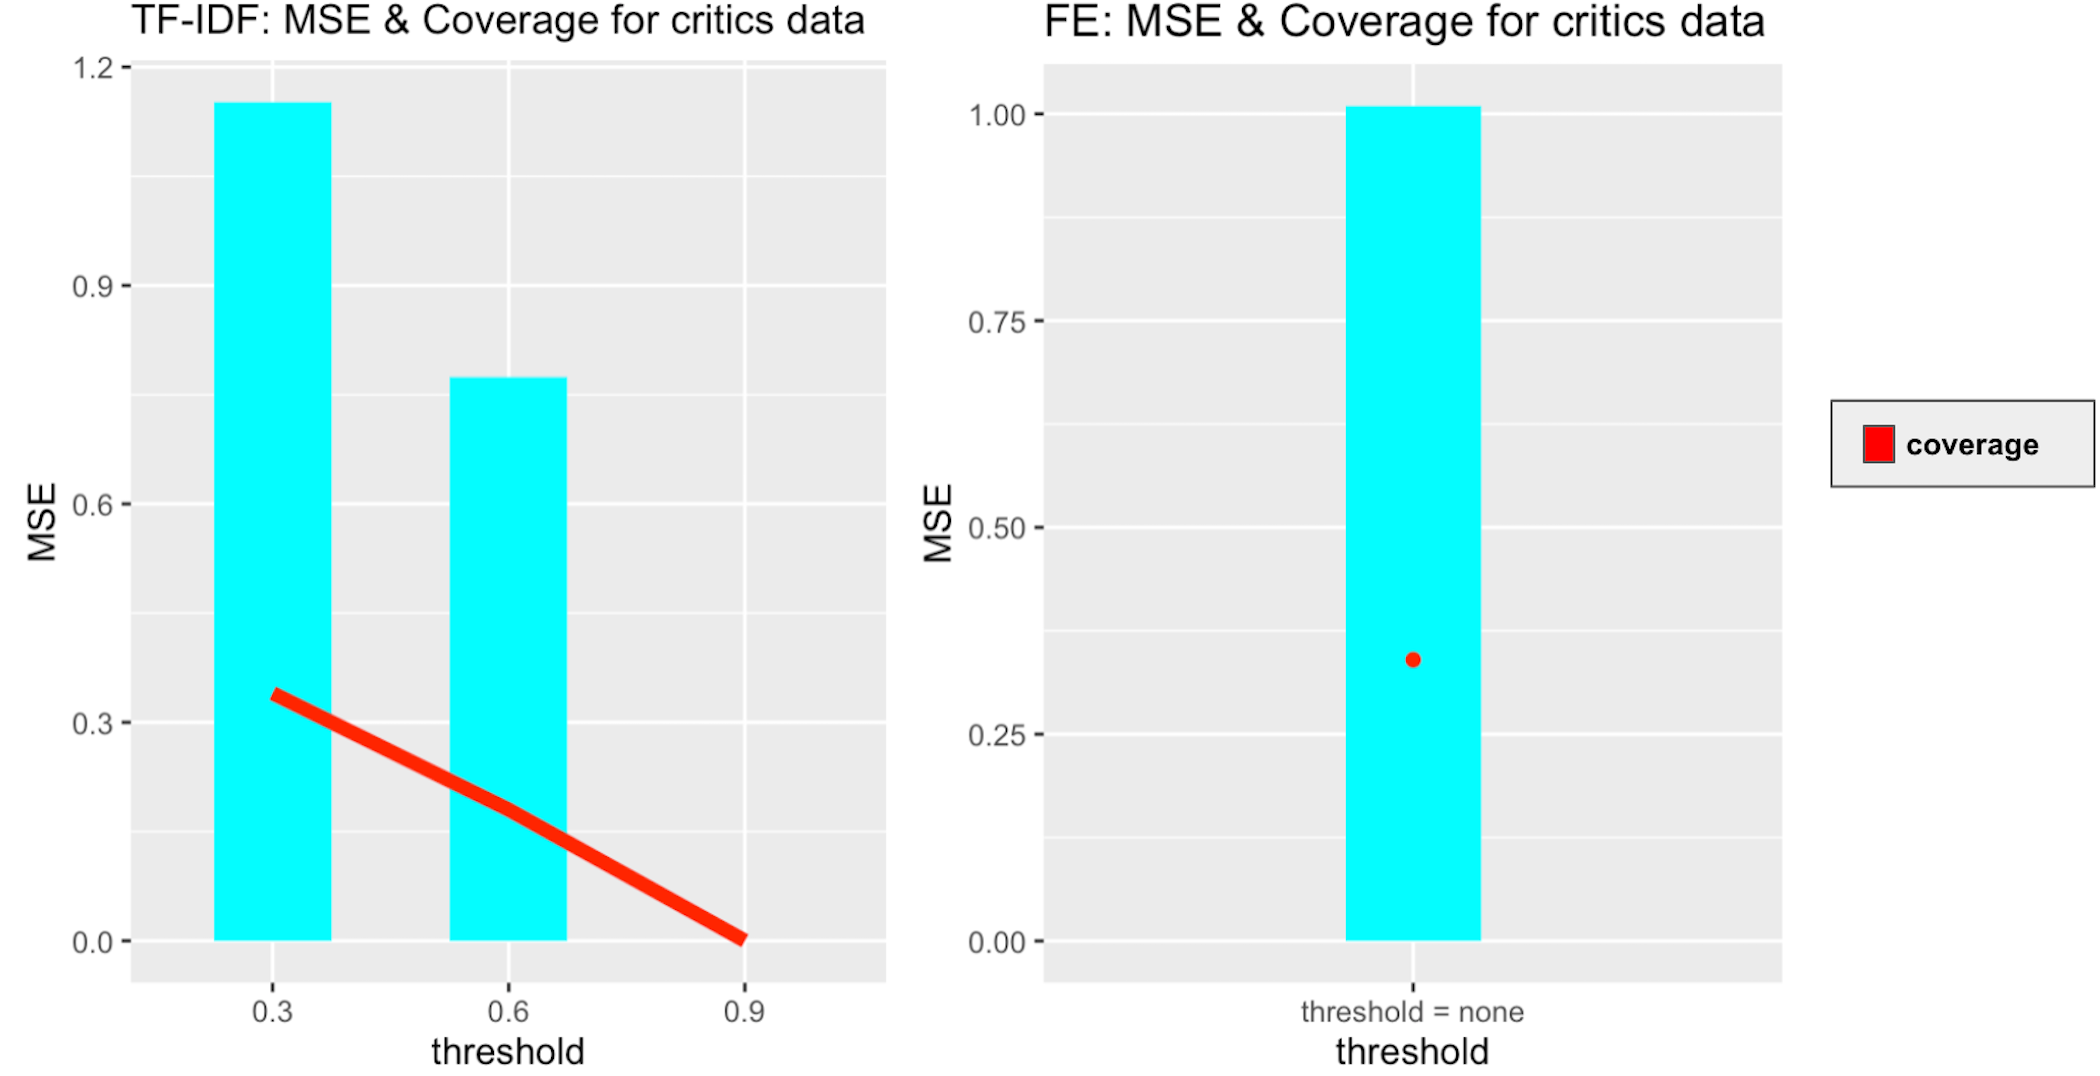
\includegraphics[width=5in]{tfidf-critics.png}
        \caption{}
        \Description{}
    \end{figure}  
    \begin{figure}[H]
        \centering
        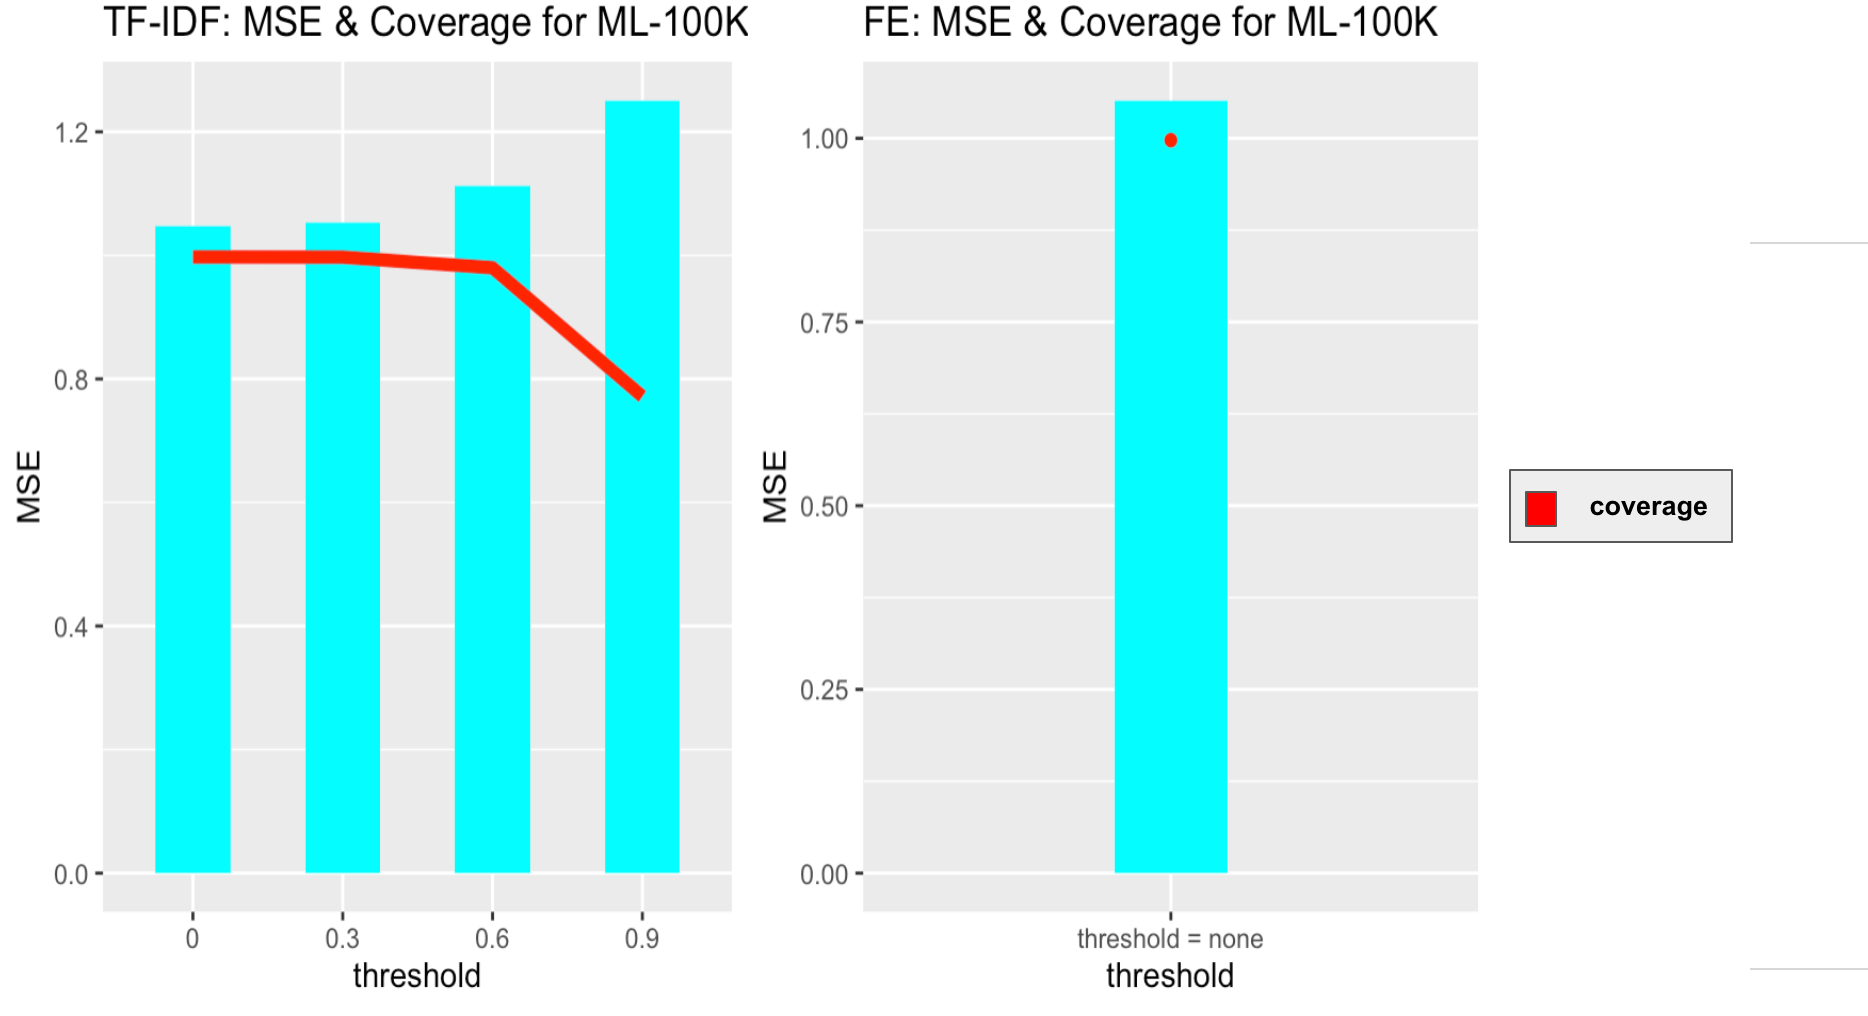
\includegraphics[width=5in]{tfidf-ml100k.png}
        \caption{}
        \Description{}
    \end{figure}  
     \begin{figure}[H]
        \centering
        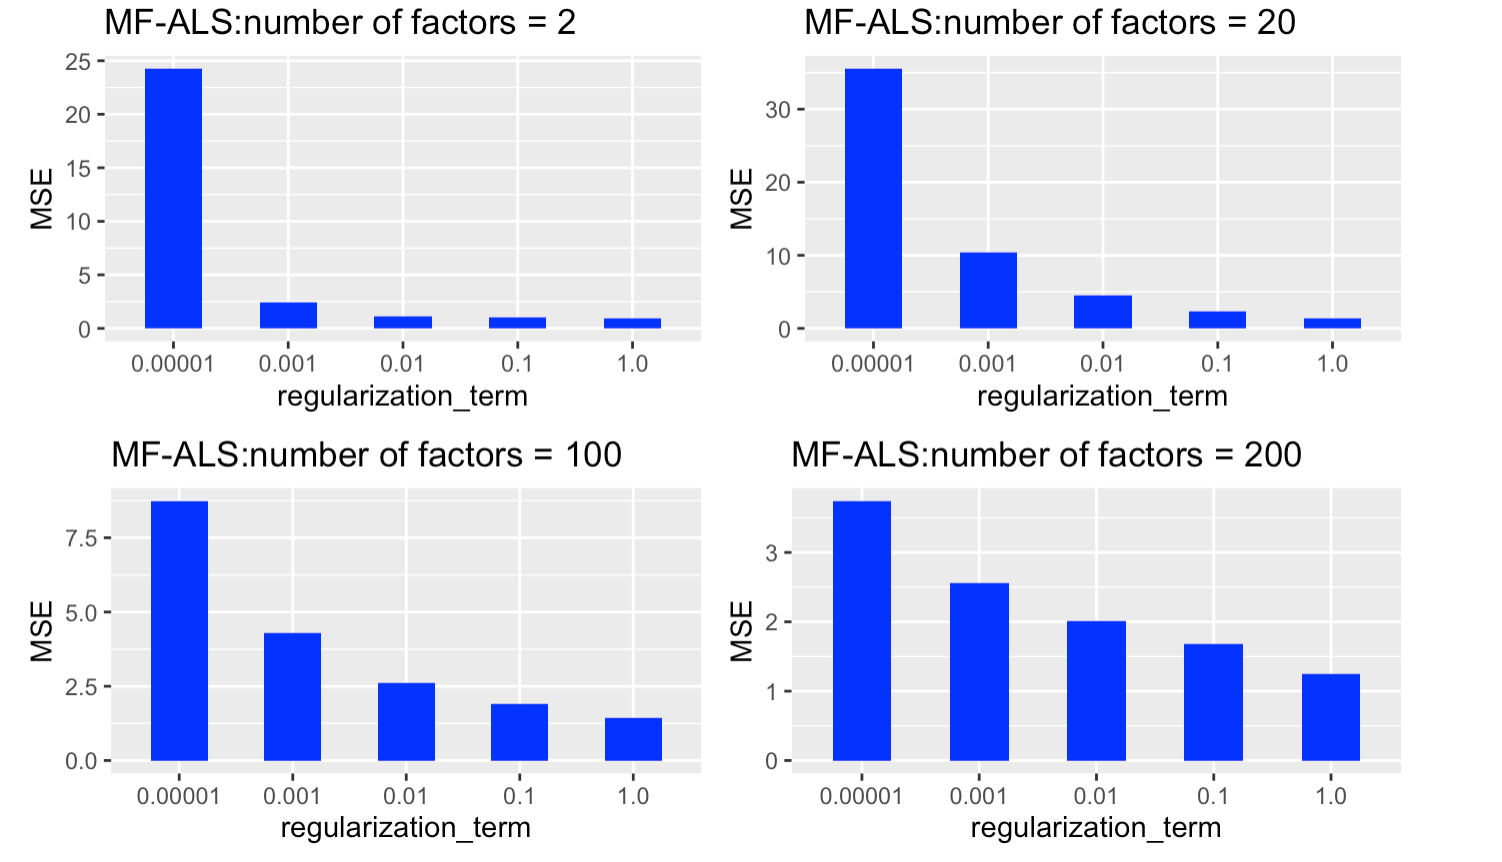
\includegraphics[width=5in]{MF-ALS.png}
        \caption{}
        \Description{}
    \end{figure}  
     \begin{figure}[H]
        \centering
        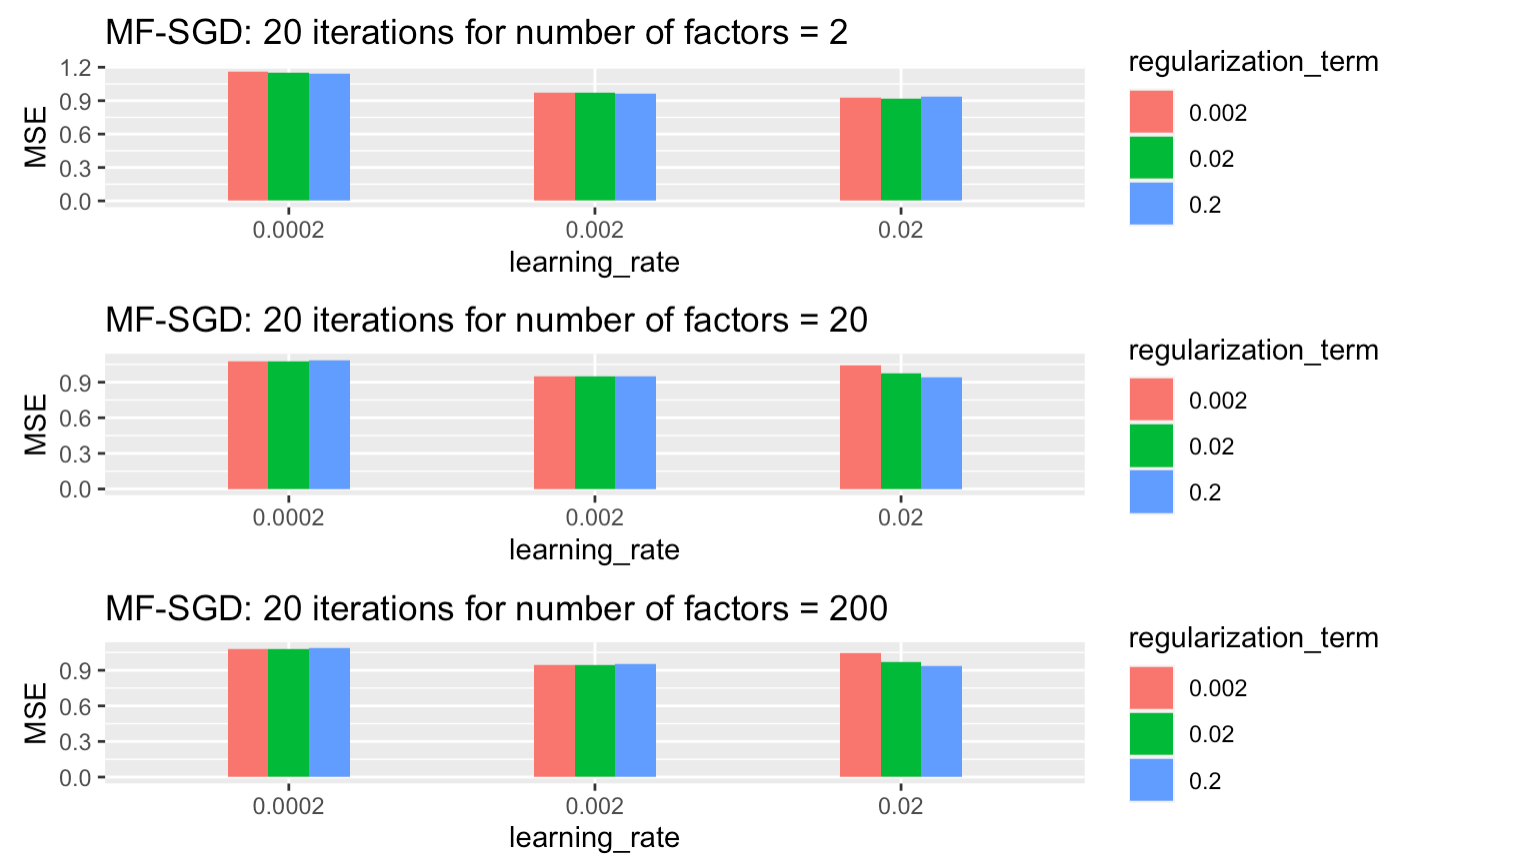
\includegraphics[width=5in]{MF-SGD.png}
        \caption{}
        \Description{}
    \end{figure}  
     \begin{figure}[H]
        \centering
        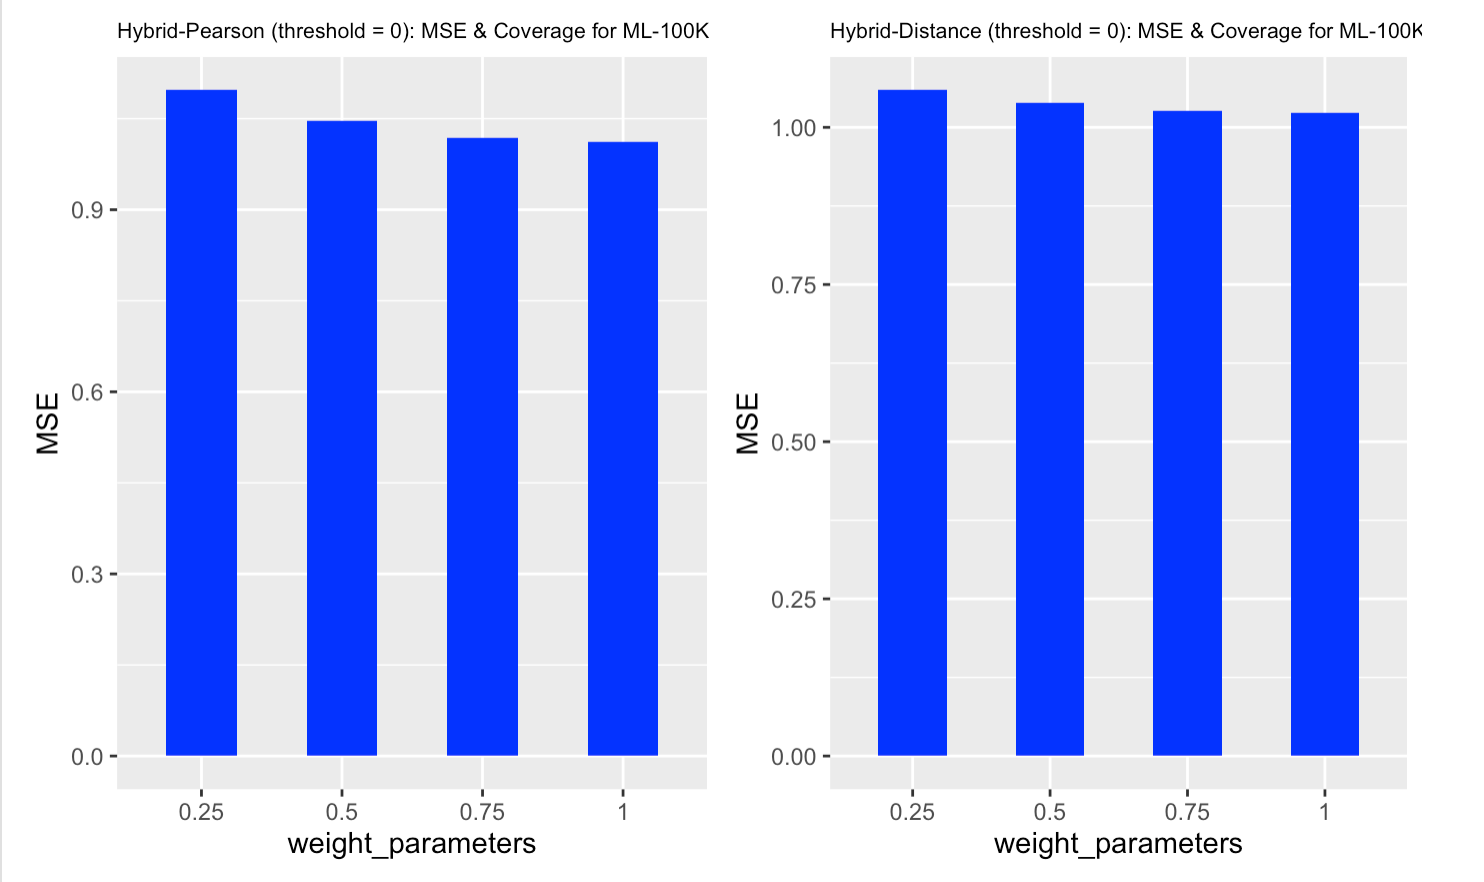
\includegraphics[width=5in]{hybrid.png}
        \caption{}
        \Description{}
    \end{figure} 
    

  
\subsection{Choosing The Best Set Of Parameters For Each Algorithm}

With regards to user-based collaborative filtering algorithms, we decided that the best set of parameters would be the similarity threshold of 0 and the significant weighting of 25 for both Pearson and Distance algorithms. The findings in our earlier research highlight a strong negative correlation between the similarity threshold value and coverage\cite{mid}. Increasing the significant weighting from 0 to 0.3, and then to 0.5, dramatically decreases the coverage of our results, hence reducing the reliability of the MSE value\cite{mid}. Therefore, a similarity threshold of 0 would ensure a low MSE and a high coverage. In addition, higher significant weighting seems to increase coverage significantly while increasing MSE by a little bit, so we choose a significant weighting of 25 to balance out the increase in coverage and increase in MSE\cite{mid}.

For item-based collaborative filtering algorithms, we notice the same patterns as user-based CF, where increasing the significant weighting from 0 to 0.3, and then to 0.6, dramatically decreases the coverage of our results, till the point of 0 for Distance\cite{mid}. The significant weighting increases coverage and decreases MSE\cite{mid}. Therefore, we decided to go with a similarity threshold of 0 and significant weighting of 25 for both Pearson and Distance algorithms.

In TFIDF algorithm, we notice that the higher threshold value is, the higher MSE (Figure 3). Therefore, we decided to go with the threshold value of 0 for the algorithm.

In terms of MF-SGD algoritm, across all three numbers of iterations, learning rate value alpha = 0.02 produces the lowest MSE results (Figure 5). As alpha decreases, MSE increases (Figure 5). Number of factors = 2 and alpha = 0.0002 produces the highest MSE (Figure 5). In addition, big values of factors also require a higher value of regularization. As regularization goes down, it is more likely that the algorithm will overfit data (Figure 5). Therefore, we decided that the best set of hyper-parameters for SGD is k = 2, alpha = 0.02, beta = 0.02 because it outputs considerably low MSE and does not overfit data.

For ALS algorithm, as regularization goes down, it is more likely that the algorithm will overfit data (Figure 4). In addition, big values of factors also require a higher value of regularization (Figure 4). Therefore, we think that the best set of hyper-parameters for ALS is k = 2, beta = 1.0. The set produces a low MSE of 0.9264 and does not overfit data.

For hybrid algorithms, we chose the TFIDF threshold of 0 for both Hybrid-Pearson and Hybrid-Distance because it is the best parameter for the algorithms as explained above. We tested our data on different weight parameter, and our findings shows that a higher value of weight parameter output higher MSE, which is the case for both Hybrid-Pearson and Hybrid-Distance (Figure 6). Therefore, we decided to go with a weight-parameter of 1 for both hybrid algorithms.


%\subsubsection{\textbf{Datasets}}

%\subsubsection {\textbf{Layout of dataset statistics}}
% -- Total number of users, items, ratings
% -- Overall average rating, standard dev (all users, all items)
% -- Average item rating, standard dev (all users)
% -- Average user rating, standard dev (all items)
% -- Matrix ratings sparsity
% -->> Average number of ratings per user, standard dev (all users)
% -->> Min, Max, Median number of ratings per user
% -- Ratings distribution histogram (all users, all items) figure.

% Popular items analytics data/Chart for ml-100K: 
% -- popular items: most rated (sorted by # ratings)
% -- popular items: highest rated (sorted by avg rating)
% -- popular items: highest rated items that have at least a "threshold" number of ratings

\section{Results}
% Provide text, charts, and tables that indicate/explain the results that were obtained by executing the Experimental Design. {\color{blue}\textbf{You do not need to report on critics dataset results!}}  These are the experimental variations with Dataset=ML-100k, Rating Prediction=Weighted:
After selecting the best set of parameters for each of our algorithms as explained in our experimental design, we conducted a comparison of the accuracy and performance between each algorithm to determine the best recommender system approach. For the next step in our analysis, across the best parameters for each algorithm, we selected the best performing variation for each of the four approaches: user and item-based collaborative filtering, collaborative filtering using matrix factorisation, content-based filtering and hybrid method. 

For collaborative filtering, our results demonstrate that item-Pearson and item-distance produce the lowest MSE (Fig. 6). It is also important to note that the coverage of both item-based algorithms does not differ significantly. 

For model-based methods using matrix factorisation, our results demonstrate that both SGD and ALS perform very similarly but matrix factorisation using stochastic gradient descent algorithm produces a slightly lower MSE (Fig. 7). 

For content-based methods,our results demonstrate that both FE and TFIDF perform very similarly but TFIDF algorithm shows  better accuracy with a slightly lower MSE (Fig. 8). 

For our hybrid approaches, hybrid method using item-pearson demonstrates better accuracy and a slightly higher coverage .(Fig. 9).


\subsection{Results Charts}
   \begin{figure}[h!]
        \centering
        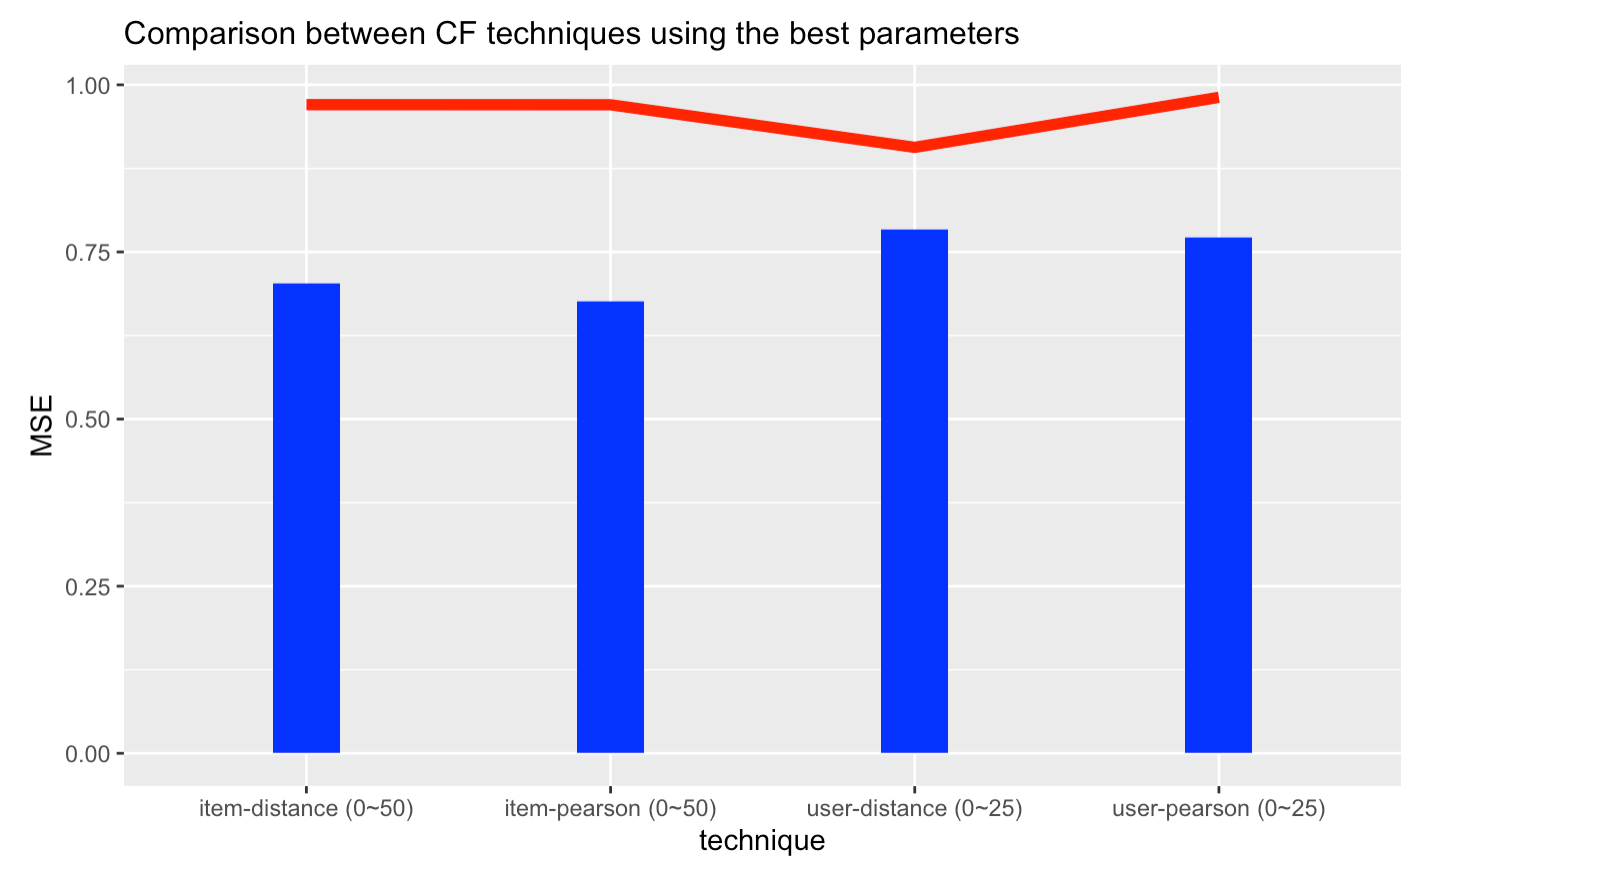
\includegraphics[width=5in]{CF.png}
        \caption{}
        \Description{}
    \end{figure}  
    \begin{figure}[h!]
        \centering
        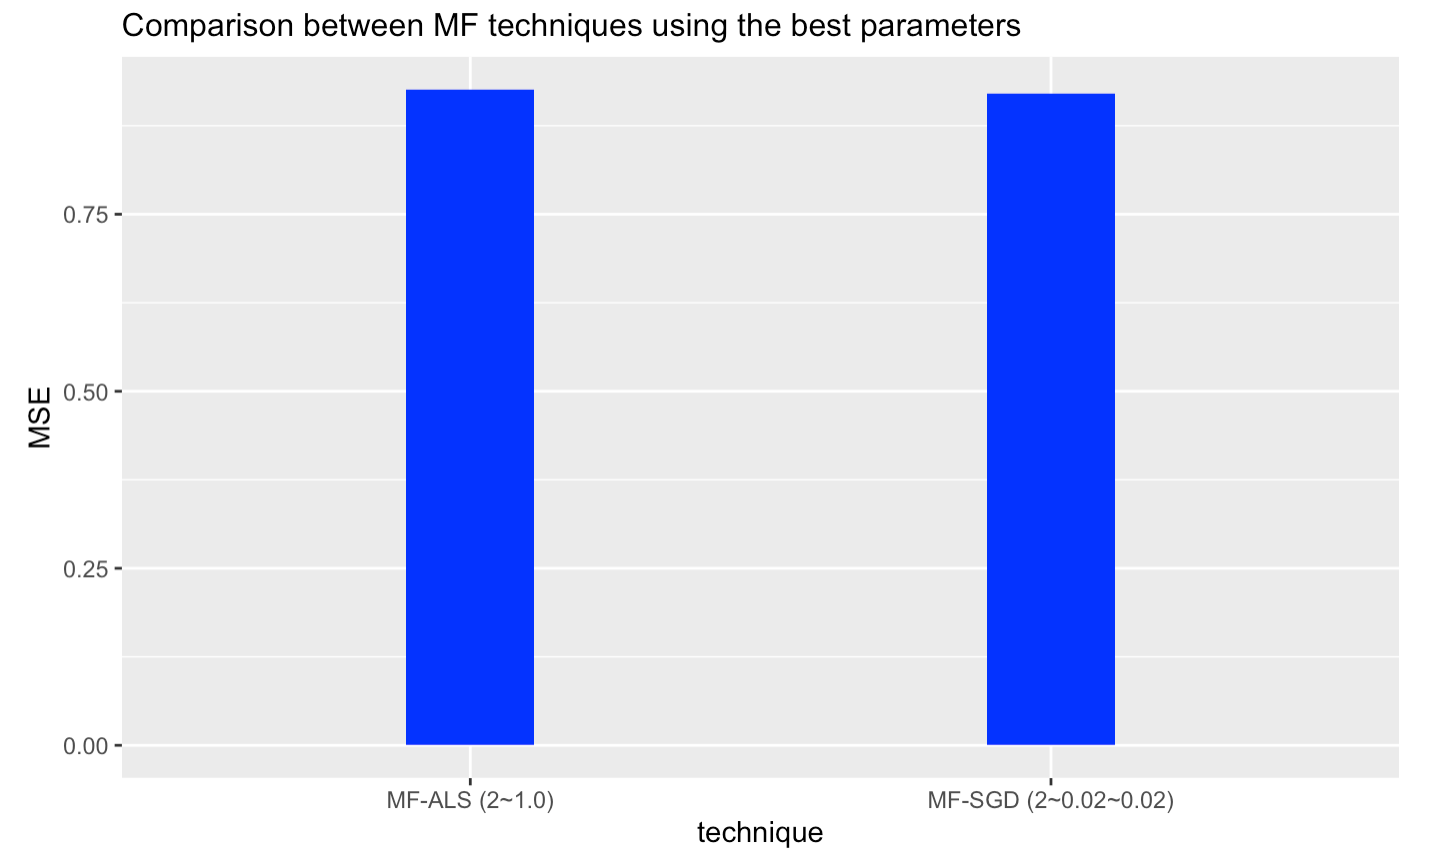
\includegraphics[width=5in]{MF.png}
        \caption{}
        \Description{}
    \end{figure}  
     \begin{figure}[h!]
        \centering
        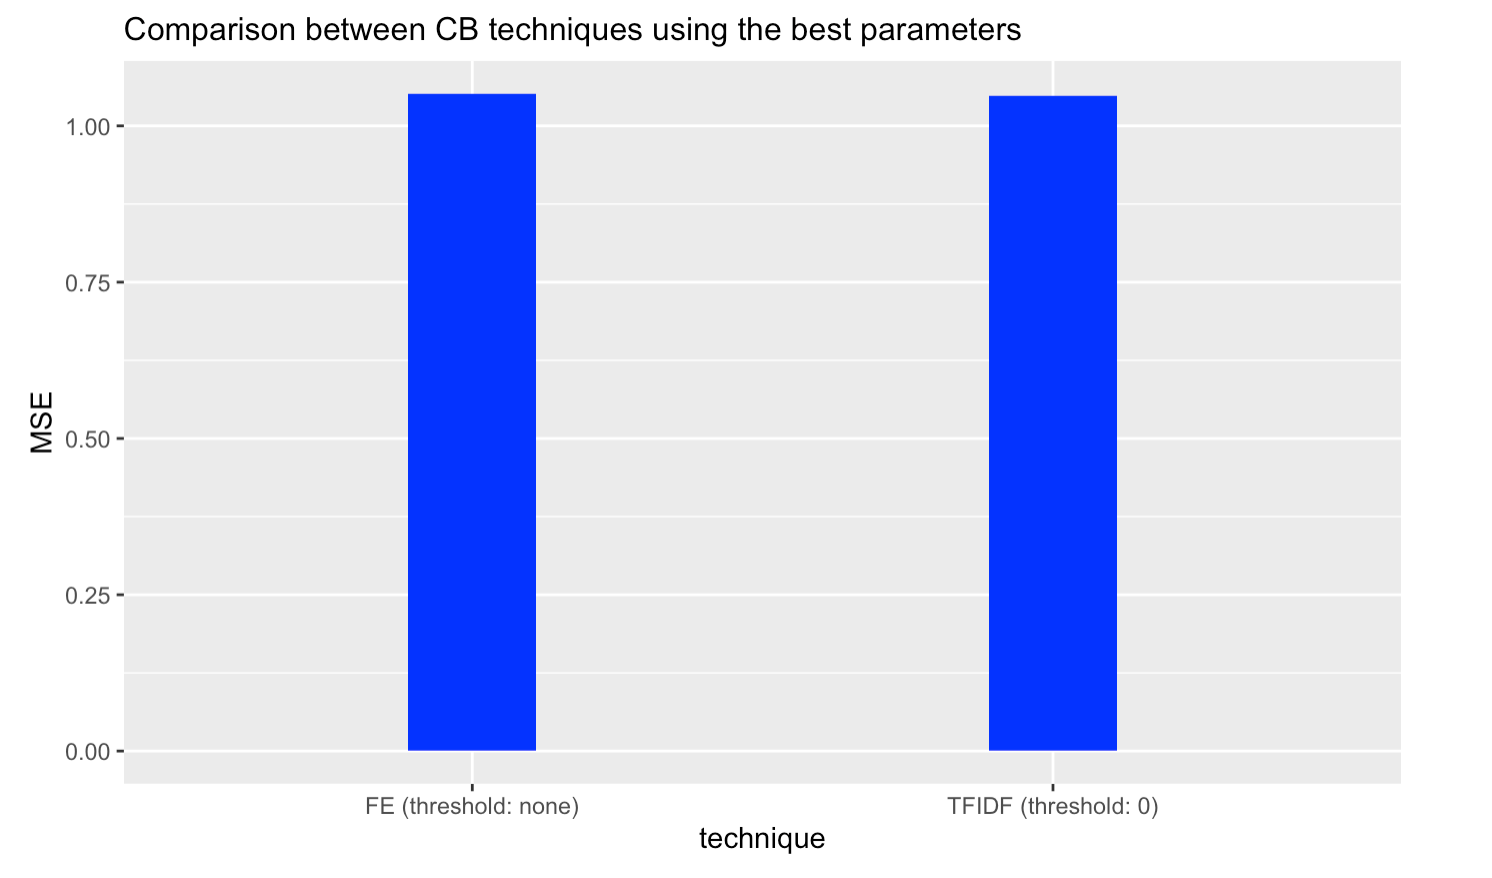
\includegraphics[width=5in]{CB.png}
        \caption{}
        \Description{}
    \end{figure}  
     \begin{figure}[h!]
        \centering
        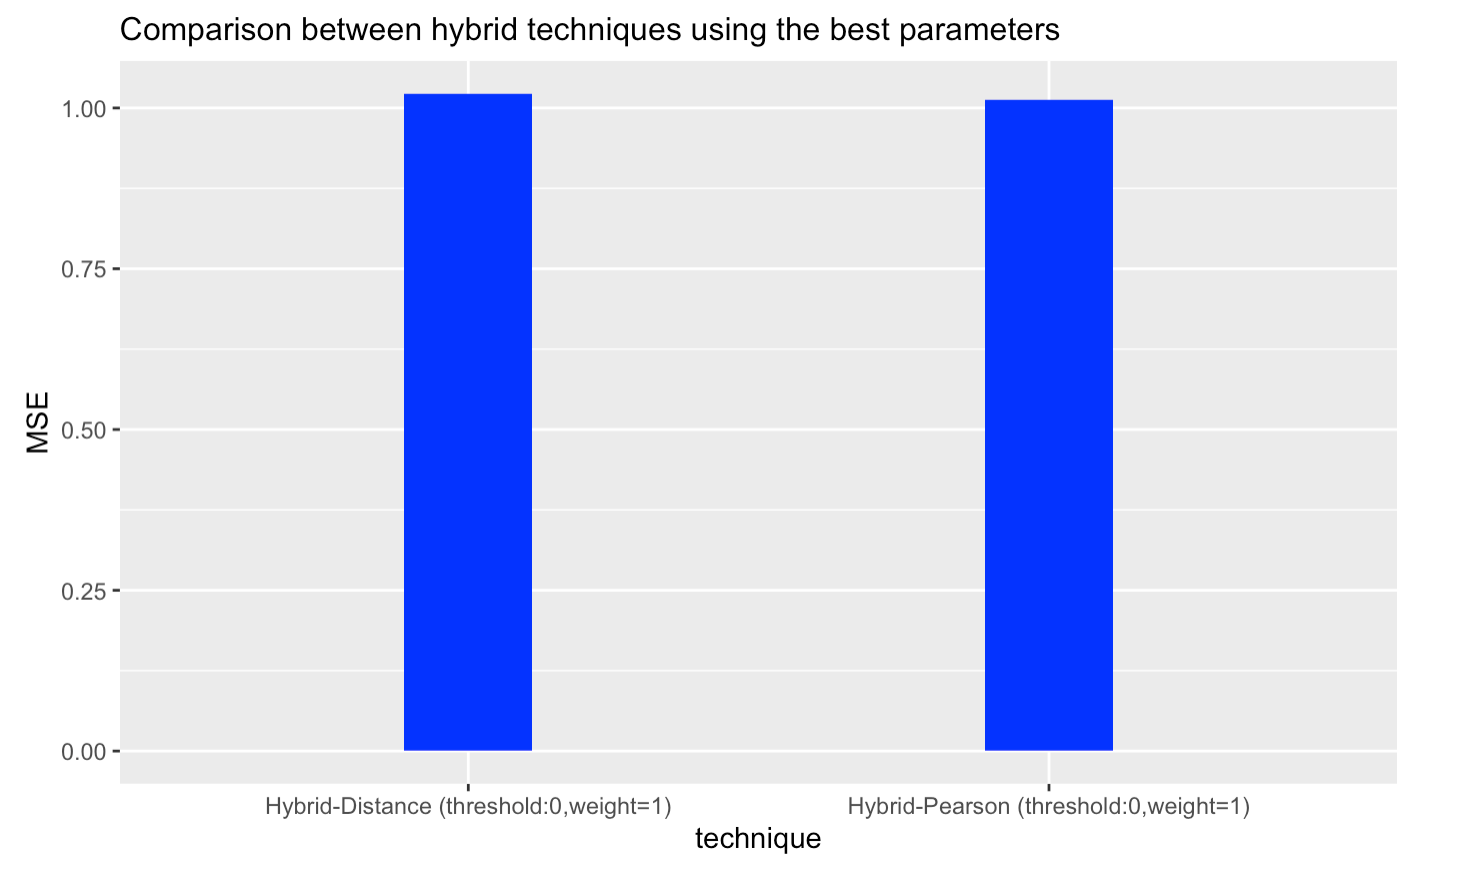
\includegraphics[width=5in]{hyb.png}
        \caption{}
        \Description{}
    \end{figure}  
     \begin{figure}[h!]
        \centering
        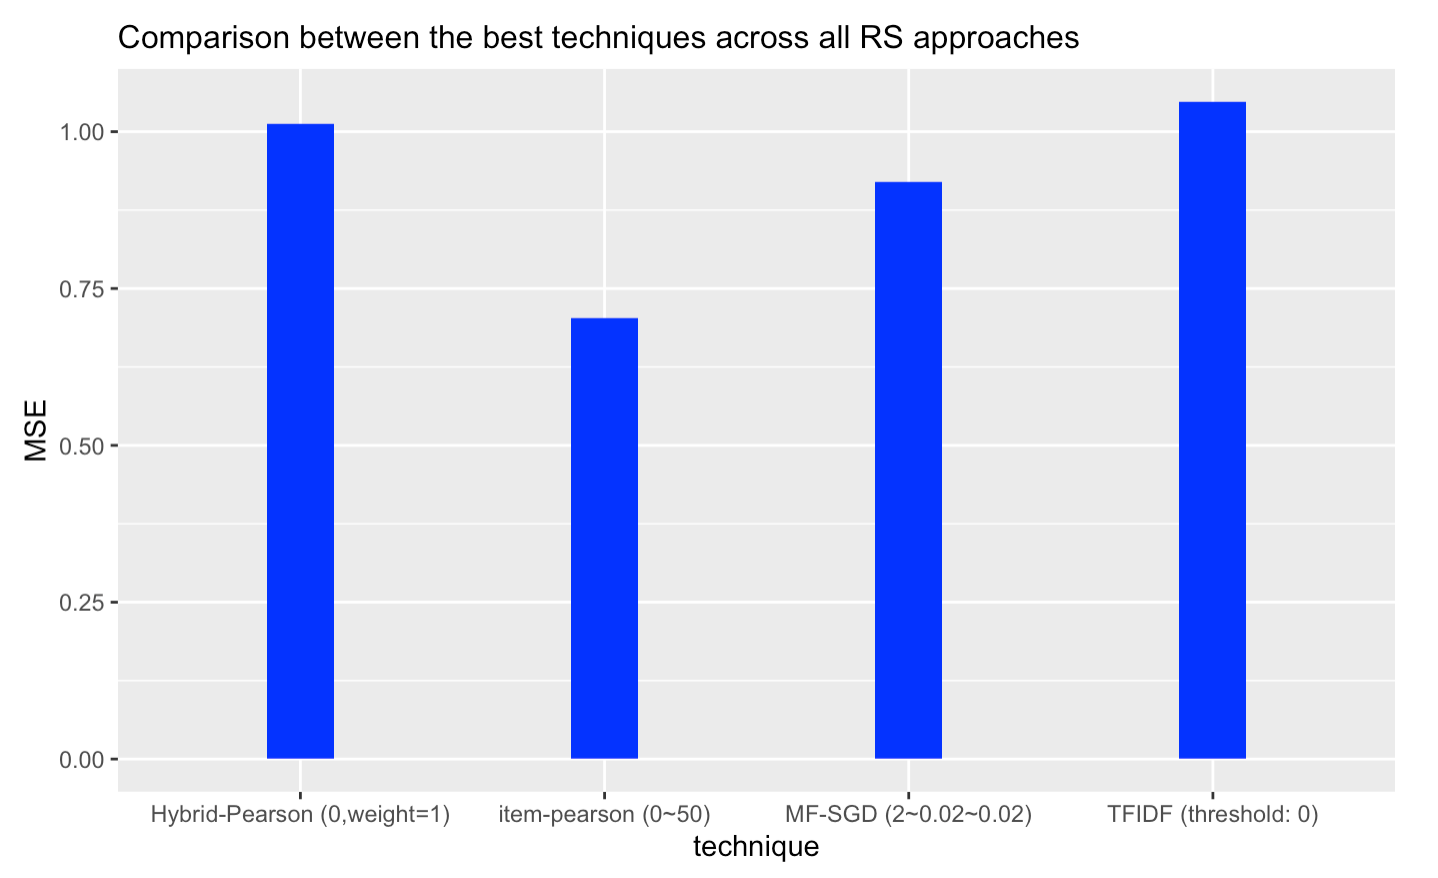
\includegraphics[width=5in]{best.png}
        \caption{}
        \Description{}
    \end{figure} 
       \begin{figure}[h!]
        \centering
        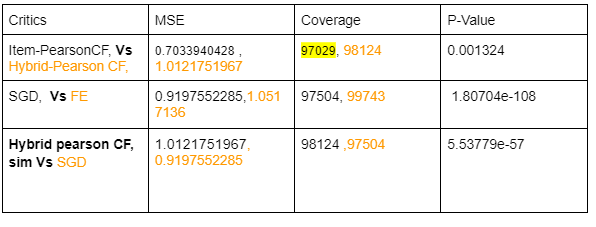
\includegraphics[width=5in]{t_test_two.PNG}
        \caption{}
        \Description{}
    \end{figure} 
    
% \pagebreak

\section{Discussion}
According to our results in Fig. 6, item-based pearson showed better accuracy than item-based distance. Therefore, we selected item-pearson as the better memory-based collaborative filtering. Our selection corresponds with the findings in previous research conducted on different similarity weighting measures, where Pearson outperformed all variants tested (Herlocker et al ., 1999).

Fig. 7 indicates that model-based method SGD and AlS perform equally well in terms of accuracy. However, SGD is a better performing algorithm because it is generally easier and faster to implement. Moreover, ALS is more preferable when the system includes more implicit data which is not the case for our RML-100K dataset because it has lower sparsity. 

Fig. 8 indicates that TF-IDF is a more accurate content-based algorithm. Feature analysis using feature encoding can be less accurate because every feature might not have similar importance (Seminario slides). Moreover, the features must be easily parsed or manually assigned to each item which proves to be a more time-consuming process (Adomavicius 2005). 
Fig.9 is comparing all the best techniques show that item-based distance and mf-sgd perform significantly better than hybrid-pearson and tfidf in terms of accuracy. Even though that item-based distance perform better than mf-sgd, we believe that mf-sgd will surpass item-based distance in the long run. Since mf-sgd allows for the incorporation of a much more in-depth dataset of information: explicit feedback, implicit feedback, biases, dynamics along with confidence levels. The prediction of calculation is based on more subtle and complex feature dimensions that Item-based CF methods won’t be able to spot. As more data is collected, mf-sgd will definitely output better recommendations. Therefore, we choose SGD as our best recommender system.

Our final table compares the 4 techniques using t-test to determine if there is a significant difference between the means of two groups, which may be related in certain features.
After comparing all the four elements as shown in fig 11. We can deduce that the mean squared errors between item-pearson and MF-SGD are different. 

We select MF-SGD because it has a relatively low MSE and offers a compact memory-efficient model that systems can learn relatively easy.Additionally, it can integrate naturally many crucial aspects of the data such as multiple forms of feedback, temporal dynamics and confidence levels \cite{koren}.
 
\section{Conclusion}
Overall, the findings confirmed our original hypothesis, with MF-SGD recommender systems outputting the best accuracy and coverage. We acknowledge that there are still many opportunities for further analysis following the footsteps of our work. First, there are potentially many recommender systems that have not been covered in our study, such as demographic, utility-based and knowledge-based techniques along with a substantial number of different hybrid models\cite{burke}. We plan to further extend our study by providing a comprehensive analysis of a wider range of recommender systems with the incorporation of the above-mentioned methods. In addition, one limitation of our study is that the dataset that we test our algorithms on is solely for movies. Each algorithm may perform differently when dealing with different domains of data. There are different domains that we look forward to performing our algorithms on, such as books and food data. Another important point is that our dataset is static, so we would also want to explore how algorithms deal with a dynamic dataset that has ratings constantly being updated. Finally, one of the metrics that we haven’t touched on in our study is the runtime of our algorithm. When dealing with big data, the element of runtime requires utmost attention. Therefore, we want to further extend our study with our algorithms’ runtime as one of the main metrics for our analysis.
\section{Acknowledgments}

We are grateful to our CSC 381 professor Dr. Carlos Seminario who personally worked with us to help us navigate through the challenges in the project. We are also grateful to the authors of our cited related research works because of how their ideas have helped us shaped our own research. 

\begin{thebibliography}{widest entry}
 \bibitem{her99} Jonathan L. Herlocker, Joseph A. Konstan, Al Borchers, John Riedl,  \emph{An Algorithmic Framework for Performing Collaborative Filtering}, 1999
 \bibitem{bad} Badrul Sarwar, George Karypis, Jospeph Konstan, and John Riedl, \emph{Item-Based Collaborative Filtering Recommendation Algorithms}, 2001
 \bibitem{car} Carlos Seminario, \emph{Moodle Slides}, 2022
 \bibitem{par} Parul Pandey, \emph{The Remarkable World of Recommender Systems}, 2019
 \bibitem{koren} Koren et al, \emph{Matrix Factorization Techniques for Recommnder Systems}, 2009
 \bibitem{pazz} Pazzani Billsus, \emph{Content-Based Recommendation Systems}, 2007
 \bibitem{adoma} G. Adomavicius, \emph{Toward the Next Generation of Recommender Systems}, 2005
 \bibitem{burke} Burke, \emph{Hybrid Recommender Systems: Survey and Experiments}, 2002
 \bibitem{movie} F.M. Harper and J.A.Konstan, \emph{The MovieLens Datasets: History and Context}, 2016
 \bibitem{des} Desrosiers/Karypis, \emph{A comprehensive survey of neighborhood-based
recommendation methods}, 2011
\bibitem{zhou} Zhou, \emph{Large-scale Parallel Collaborative Filtering for the Netflix Prize}, 2008

\bibitem{mid} Hoang, Wang, Remezo, Kalani, \emph{Impact of Variations of Similarity and Prediction Techniques on User-based and Item-based Collaborative Filtering Recommendations}, 2022
 

 

 
 

\end{thebibliography}


\newpage

%%
%% The next two lines define the bibliography style to be used, and
%% the bibliography file.
%\bibliographystyle{ACM-Reference-Format}
%\bibliography{sample-base}









\end{document}
\endinput
%%
%% End of file `sample-manuscript.tex'.
